\mode*

%\newmintedfile{java}{frame=single,linenos,samepage}

% =============================================================================
%                                 CHAPTER
% =============================================================================


\section{Modulidentifikation}
\label{sec:identification}

Für unsere Lernziele richten wir uns nach den Vorgaben des Verbandes
\href{https://ict-berufsbildung-bern.ch}{ICT Berufsbildung Bern} und hier im Spezifischen
nach den Kompetenzanforderungen für das
\href{https://cf.ict-berufsbildung.ch/modules.php?name=Mbk&a=20101&cmodnr=404&noheader=1}
{Modul 404}.

\begin{frame}[fragile]
    \frametitle<presentation>{Handlungsziele}

    \begin{enumerate}
        \item Aufgrund einer Vorgabe den Ablauf darstellen.
        \item Eine Benutzerschnittstelle entwerfen und implementieren.
        \item Erforderliche Daten bestimmen und Datentypen festlegen.
        \item Programmvorgabe unter Nutzung vorhandener Komponenten mit deren Eigenschaften und Methoden, sowie
        Operatoren und Kontrollstrukturen implementieren.
        \item Beim Programmieren vorgegebene Standards und Richtlinien einhalten, das Programm inline dokumentieren und
        dabei auf Wartbarkeit und Nachvollziehbarkeit achten.
        \item Programm auf Einhaltung der Funktionalität testen, Fehler erkennen und beheben.
    \end{enumerate}

\end{frame}


% =============================================================================
%                                 CHAPTER
% =============================================================================

\section{Bereitsstellen der Software}
\label{sec:java-technologie}

Java ist eine Programmiersprache und Computerplattform, die erstmals 1995 von
Sun Microsystems veröffentlicht wurde. Es gibt viele Anwendungen und
Websites, die nicht funktionieren, es sei denn, Sie haben Java installiert,
und jeden Tag werden weitere erstellt. Java ist schnell, sicher und
zuverlässig. Von Laptops bis hin zu Rechenzentren, Spielkonsolen bis hin zu
wissenschaftlichen Supercomputern, Handys bis hin zum Internet.

Am 20. April 2009 kündigte Oracle die Übernahme von Sun Microsystems für
7,4 Milliarden US-Dollar an, welche in den Folgemonaten durch verschiedene
Behörden überprüft und anschliessend genehmigt wurde.

Java als Entwicklungs- und Laufzeitumgebung kann in verschiedenen Varianten
von den folgenden Seiten heruntergeladen und installiert werden:


\subsection{Installation der Umgebung}
\label{subsec:installation}

\begin{frame}[fragile]
    \frametitle<presentation>{Installation der Umgebung}

    Wir unterscheiden im Wesentlichen zwischen den beiden Installationstypen
    JRE ({\em Java Runtime Environment}) und JDK ({\em Java
    Development Kit}).

    Die wichtigsten {\em Links} zu diesen Umgebungen finden wir hier:

    \begin{itemize}
        \item \href{https://java.com}{java.com}
        \item \href{https://openjdk.java.net}{openjdk.java.net}
    \end{itemize}

\end{frame}

In der Softwareentwicklung konzentrieren wir uns ausschliesslich auf das JDK,
da wir auf die vielen zusätzlichen {\em Tools} in der Entwicklung angewiesen
sind.


\begin{frame}[fragile]
    \frametitle<presentation>{Werkzeuge und Befehle}

    Die JDK-Tools und ihre Befehle ermöglichen es uns,
    Entwicklungsaufgaben wie das Kompilieren und Ausführen eines Programms,
    das Paketieren von Quelldateien und vieles mehr zu erledigen.

    \mode<presentation>{Hier nur eine kleine Auswahl:}
    \begin{itemize}
        \item\href{https://docs.oracle.com/en/java/javase/11/tools/javac.html}
        {javac}---Kompilieren von Klassen- und Schnittstellendefinitionen
        in Bytecode.
        \item\href{https://docs.oracle.com/en/java/javase/11/tools/java.html}
        {java}---Starten/Interpretieren eines Java Programms.
        \item\href{https://docs.oracle.com/en/java/javase/11/tools/jar.html}
        {jar}---Erstellen eines Java Archives.
        \item\href{https://docs.oracle.com/en/java/javase/11/tools/jshell.html}
        {jshell}---Interaktives Auswerten von Deklarationen, Anweisungen und
        Ausdrücken der Programmiersprache Java.
        \item<article>\href{https://docs.oracle.com/en/java/javase/11/tools/javap.html}
        {javap}---Befehl, um eine oder mehrere Klassendateien zu
        disassemblieren.
        \item<article>\href{https://docs.oracle.com/en/java/javase/11/tools/javadoc.html}
        {javadoc}---Erstellen der Java Dokumentation
        \item<article>\href{https://docs.oracle.com/en/java/javase/11/tools/keytool.html}
        {keytool}---Befehl und Optionen zum Verwalten eines kryptografischer Schlüssel.
        \item<article>\href{https://docs.oracle.com/en/java/javase/11/tools/jarsigner.html}
        {jarsigner}---Signieren und verifizieren von Java Archiven
    \end{itemize}

\end{frame}


Diese Liste stellt keinen Anspruch auf Vollständigkeit. Die komplette Dokumentation
zu den einzelnen Umgebungen und deren {\em Tools} kann jederzeit unter
\href{https://docs.oracle.com/en/java/}{docs.oracle.com} eingesehen werden.

Vorsicht ist allerdings geboten, wenn es um den Einsatz und die Lizenzierung von Java geht.
Oracle wird nach Januar 2019 keine weiteren Updates von Java SE 8 zur
gewerblichen Nutzung auf seinen Download-Sites veröffentlichen. Kunden, die
weiterhin Zugriff auf kritische Fehlerkorrekturen und Sicherheitslücken sowie
eine allgemeine Wartung von Java SE 8 bzw. früheren Versionen benötigen,
können einen langfristigen Support über Oracle Java SE Advanced erhalten.
Oracle Java SE Advanced Desktop oder Oracle Java SE Suite. Für weitere
Informationen und Details, wie Sie einen längerfristigen Support für Oracle
JDK 8 erhalten, finden Sie in der
\href{http://www.oracle.com/technetwork/java/eol-135779.html}
{Oracle Java SE Support-Roadmap}.

Die offizielle \href{https://www.oracle.com/corporate/pricing/#java-se}
{Preisliste} hilft, sich mit dem Oracle Java SE Abonnement für On Premise,
Enterprise, Desktop, Server und Cloud Workloads vertraut zu machen.


\begin{frame}[fragile]
    \frametitle<presentation>{Beliebte Java-Lernressourcen}

    \begin{itemize}
        \item\textbf{Finch Robot}---Dieser kleine Roboter von
        \href{https://www.birdbraintechnologies.com/finch/}
        {Bird Technology} nutzt verschiedene Sensoren,
        die via Java angesteuert werden können.
        \item\textbf{Oracle Academy}---Die
        \href{https://academy.oracle.com/en/training-self-study.html}
        {Oracle Academy} bietet verschiedene
        Online-Kurse und Anleitungen
        \item\textbf{Scratch}---Dies ist eine sehr einfache, am
        \href{https://scratch.mit.edu/}{MIT} entwickelte Programmierumgebung.
        Typischerweise wird diese im Vorschulalter eingesetzt.
        \item\textbf{BlueJ}---Als sehr professionelle und stark vereinfachte
        (Entwicklungs-) Umgebung wird \href{http://www.bluej.org/}{BlueJ}
        auch im späteren Alter noch für Schulungszwecke verwendet.
    \end{itemize}

\end{frame}


%
% In einer ersten Übung wollen wir die Java Entwicklungsumgebung installieren.
% Dies ist notwendig, dass wir die anschliessenden Beispiele gemeinsam anschauen
% und erweitern können.
%
\mode<presentation>
\begin{frame}[fragile]
    \frametitle{Übung - Installation der Software}
    Bevor wir mit unseren Übungen starten müssen wir sicherstellen,
    dass Java und seine {\em Tools} komplett und korrekt installiert sind.

    Bitte installieren Sie das {\em Java Development Kit} (OpenJDK) gemäss
    <\href{https://jdk.java.net/11/}{jdk.java.net/11}>.

    \vfill
    Anschliessende Kontrolle der Installation mit:

    \begin{minted}[frame=single,autogobble]{text}
        # java -version
        openjdk version "11.0.1" 2018-10-16
        ...
    \end{minted}

\end{frame}


\mode*

\begin{Exercise}[%
title={Installation der Software},
label={ex:installation}]

    Bevor wir mit unseren Übungen starten müssen wir sicherstellen, dass Java und
    seine {\em Tools} komplett und korrekt installiert sind.

    Bitte installieren Sie das {\em Java Development Kit} (OpenJDK) gemäss
    \href{https://jdk.java.net/11/}{Anleitung}.

    Anschliessend überprüfen wir die korrekte Installation mit Hilfe der Konsole wie folgt:

    \begin{minted}[frame=single,autogobble]{text}
        # java -version
        openjdk version "11.0.1" 2018-10-16
        OpenJDK Runtime Environment 18.9 (build 11.0.1+13)
        OpenJDK 64-Bit Server VM 18.9 (build 11.0.1+13, mixed mode)
    \end{minted}

\end{Exercise}

\subsection{Interaktive Entwicklungsumgebung}
\label{subsec:ide}

Jeder Java-Entwickler benötigt einen Programmiereditor oder eine IDE, der bei den
grungierigeren Teilen des Schreibens von Java und der Verwendung von Klassenbibliotheken
und Frameworks helfen kann. Die Entscheidung, welche IDE zum Einsatz kommt, hängt von
mehreren Faktoren ab, darunter der Art der zu entwickelnden Projekte, dem vom
Entwicklungsteam verwendeten Prozess sowie dem Niveau und den Fähigkeiten des
Entwicklers. Weitere Überlegungen sind, ob das Team die Tools und Ihre persönlichen
Präferenzen standardisiert hat.


\begin{frame}[fragile]
    \frametitle<presentation>{Entwicklungsumgebungen}

    Die drei am häufigsten für die Java-Entwicklung gewählten IDEs sind

    \begin{itemize}
        \item \href{https://www.jetbrains.com/idea}{IntelliJ IDEA}
        \item \href{https://www.eclipse.org/}{Eclipse}
        \item \href{https://netbeans.org/}{NetBeans}
    \end{itemize}

\end{frame}


Ein guter Vergleich dieser drei Umgebungen ist auch
\href{https://www.javaworld.com/article/3114167/development-tools/choosing-your-java-ide.html}
{hier} zu finden. Persönlich habe ich Eclipse in den Anfängen der IDE, später
NetBeans in den Schulungen und zu guter Letzt IntelliJ IDEA verwendet. Nach
jedem Wechsel spürte ich, dass sich meine Produktivität verbessert hatte.

Ich habe mich für IntelliJ IDEA Ultimate entschieden. Obwohl es nicht kostenlos
wie Eclipse oder NetBeans ist, glaube ich, dass der Produktivitätsgewinn den
Preis wert ist. Für unsere Schulung ist es allerdings unerheblich, welches
Produkt wir einsetzten, auch wenn ich bestimmt mit IntelliJ IDEA die bessere
Unterstützung bieten kann.


\mode<presentation>
\begin{frame}[fragile]
    \frametitle<presentation>{Übung - Installation der Entwicklungsumgebung}

    Ich habe mich für IntelliJ IDEA Ultimate entschieden. Obwohl es nicht kostenlos
    wie Eclipse oder NetBeans ist, glaube ich, dass der Produktivitätsgewinn den
    Preis wert ist.

    Für die Ausbildung können wir die Umgebung allerdings kostenfrei nutzen.

    Installiert kann diese Software via <\href{https://www.jetbrains.com/idea/download}
    {www.jetbrains.com/idea/download}>

\end{frame}

\begin{frame}[fragile]
    \frametitle<presentation>{Übung - Eingeben der Lizenz}

    \begin{minipage}[b]{0.5\textwidth}
        \image{intellij-license}{IntelliJ IDEA Lizenz}
    \end{minipage}
    \begin{minipage}[b]{0.4\textwidth}
        Während der Dauer dieser Ausbildung dürfen wir die Schulungslizenz
        kostenfrei nutzen.

        \parskip1em
        Wir referenzieren an dieser Stelle eine sogenannte {\em floating license},
        die uns von der Talent Factory zur Verfügung gestellt wurde.
    \end{minipage}

\end{frame}


\mode*
\begin{Exercise}[%
title={Installation der Entwicklungsumgebung},
label={ex:installation-intellij}]

    Für die Entwicklung und die Zusammenarbeit mit dem vorhandenen Git \emph{Repository}
    und für die Generierung der Unterlagen (Skript und Folien) werden wir noch weitere
    Werkzeuge nutzen, die wir vorgängig installieren müssen.

    \begin{enumerate}
        \item \href{https://www.jetbrains.com/idea}{IntelliJ IDEA}. Mit dieser IDE
        machen wir unsere Entwicklungen zu einem angenehmen Erlebnis.
        \item Git für \href{https://git-scm.com/download/mac}{Mac},
        \href{https://git-scm.com/download/win}{Windows} oder
        \href{https://git-scm.com/download/linux}{Linux}.
        Mit der Versionskontrolle \href{https://git-scm.com/book/de/v2/}{Git}
        verwalten wir all unsere Dokumente wie Quellcode, Skript, Folien und
        Prüfungen.
        \item \TeX\ Live für \href{http://tug.org/cgi-bin/mactex-download/MacTeX.pkg}{Mac},
        \href{http://mirror.ctan.org/systems/texlive/tlnet/install-tl-windows.exe}{Windows} oder
        \href{http://mirror.ctan.org/systems/texlive/tlnet/install-tl-unx.tar.gz}{Linux}.
        Dies ist die Wurzel des \emph{Comprehensive \TeX\ Archive Network} Verzeichnisbaums.
        \item \href{https://www.python.org/downloads/}{Python} ist eine Programmiersprache,
        mit der Sie schneller arbeiten und Ihre Systeme effektiver integrieren können.
        \item Dies ist die Heimat von \href{http://pygments.org/}{Pygments}.
        Es handelt sich um einen generischen Syntax-\emph{Highlighter}, der für den
        Einsatz in Code-Hosting, Foren, Wikis oder anderen Anwendungen geeignet ist.
        Unterstützt werden mehr als 300 Programmiersprachen.
        \item \href{https://cygwin.com/}{Cygwin} ist eine grosse Sammlung von GNU- und
        Open-Source-Tools, die eine ähnliche Funktionalität wie eine
        Linux-Distribution unter Windows bieten.
    \end{enumerate}

\end{Exercise}

% =============================================================================
%                                 CHAPTER
% =============================================================================

\section{Objekte und Klassen}
\label{sec:contents}

\begin{frame}[fragile]
    \frametitle<presentation>{Fundamentale Konzepte}

    \begin{itemize}
        \item Klassen
        \item Objekte
        \item Eigenschaften $|$ Attribute
        \item Methoden
        \item Parameter
        \item \emph{Daten Typen}
    \end{itemize}
\end{frame}


\subsection{Objekte und Klassen}
\label{subsec:objects-classes}

Wenn Sie ein Computerprogramm in einer objektorientierten Sprache schreiben,
dann erstellen Sie im Computer ein Modell eines Auschnitts der realen Welt.
Dieser Ausschnitt setzt sich aus den \emph{Objekten} zusammen, die im
Anwendungsbereich (\emph{Problem Domain}) vorkommen.

% LaTeX uses the '~' symbol as a non-breaking space.
% https://en.wikibooks.org/wiki/LaTeX/FAQ#Non-breaking_spaces

In der Abbildung~\ref{fig:uml-class} sehen wir eine einfache Klasse,
welche im vorliegenden Fall nur aus dem Namen selbst besteht. Der Name der Klasse,
sowie alle weiteren Definitionen wie Eigenschaften (Attribute), Konstanten und Methoden
folgen einer klaren Namenskonvention, auch bekannt unter
\href{https://www.geeksforgeeks.org/java-naming-conventions/}{CamelCase}.

\begin{frame}[fragile]
    \frametitle<presentation>{Darstellung einer Klasse}

    \begin{figure}[ht]
        \centering
        \begin{minipage}[b]{0.5\textwidth}
            \centering
            \begin{tikzpicture}
                \umlclass[width=4cm]%
                {Person}{Eigenschaften}{Methoden}
            \end{tikzpicture}
        \end{minipage}
        \begin{minipage}[b]{0.4\textwidth}
            \begin{minted}[frame=single,autogobble]{java}
                public class Person {
                // Eigenschaften
                // Methoden
                }
            \end{minted}
        \end{minipage}
        \mode<article>{\caption{UML Diagramm vs Implementation}}
        \mode<presentation>{\centering UML Diagramm vs Implementation}
        \label{fig:uml-class}
    \end{figure}

\end{frame}


\begin{frame}[fragile]
    \frametitle<presentation>{Klasse vs. Objekt}

    Doch was ist eigentlich der Untersdchied zwischen Klassen und Objekten?

    \begin{description}
        \item[Objekte] stellen \emph{Dinge} aus der realen Welt oder aus einer Problemdomäne
        dar (Beispiel: ``Das weisse Auto da unten auf dem Parkplatz'').
        \item[Klassen] repräsentieren Objekte einer bestimmten Art (Beispiel: ``Auto'').
    \end{description}

\end{frame}

Objekte können klassifiziert werden als alle Objekte einer bestimmten Art und
eine Klasse beschreibt genau dies auf abstrakte Art.

Betrachten wir unsere erste Klasse---in diesem Fall unser erstes Programm---in
seiner einfachsten Form (s. Listing~\ref{lst:hello-world}, Seite~\pageref{lst:hello-world}).

\mode<presentation>
\begin{frame}[fragile]
    \frametitle<presentation>{Meine erste Java Klasse}

    \inputminted[frame=single,samepage]{java}{../java/academy/HelloWorld.java}

\end{frame}

\mode*
\begin{listing}[ht]
    \begin{center}
        \begin{minipage}{0.8\textwidth}
            \inputminted[frame=single,linenos,samepage]{java}
            {../java/academy/HelloWorld.java}
        \end{minipage}
    \end{center}
    \caption{Erstes Programm: \emph{HelloWorld}}
    \label{lst:hello-world}
\end{listing}

Typischerweise wir eine Klasse in Java in einer Datei unter dem selben Namen abgelegt.
Hierbei ist wichtig die Gross- und Kleinschreibung zu beachten.


Der Aufbau einer Java Datei kann sehr einfach durch eine Metasprache, der sogenannten
\href{https://de.wikipedia.org/wiki/Erweiterte_Backus-Naur-Form}{Erweiterte Backus-Naur-Form}
(EBNF) dargestellt werden.

\begin{listing}[h]
    \begin{center}
        \begin{minipage}{0.8\textwidth}
            \inputminted[firstline=41,lastline=46,frame=single,linenos]{antlr}{Java.g4}
        \end{minipage}
    \end{center}
    \caption{Syntaktischer Aufbau einer Java-Datei}
    \label{antlr:java-file}
\end{listing}



\begin{frame}[fragile]
    \frametitle<presentation>{Sichtbarkeit von Objekten}

    Es existiern vier unterschiedliche Zugriffsstufen für die
    Objekte (Daten und Methoden).

    \begin{table}[ht]
        \begin{center}
            \begin{tabular}{p{3cm}|c|c|c|c}
                Modifier & Class & Package & Subclass & Universe \\ \hline
                \mintinline{java}{private}   & x & & &          \\
                \texttt{default}             & x & x & &          \\
                \mintinline{java}{protected} & x & x & x &          \\
                \mintinline{java}{public}    & x & x & x & x
            \end{tabular}
        \end{center}
        \mode<article>{\caption{Sichtbarkeit von Objekten}}
        \label{tab:access-level}
    \end{table}

\end{frame}


\mode<presentation>
\begin{frame}[fragile]
    \frametitle<presentation>{Übung: Ein einfacher Taschenrechner}
    Für unsere nächste Übung erstellen wir ein neues Projekt aus einem
    \emph{Repository}. Da es sich um ein öffentliches Projekt handelt sollte
    der Zugriff auch ohne einen persönlichen Zugang möglich sein.

    Das Projekt ist unter folgendem Link zu finden.

    \href{https://github.com/dsenften/example-simple-calculator.git}
    {https://github.com/dsenften/example-simple-calculator.git}
\end{frame}

\mode*
% ----------------------------------------------------------------------------
\begin{Exercise}[%
title={Ein einfacher Taschenrechner},
label={ex:calculator}]

    \subsubsection*{Erstellen eines neuen Projektes}

    Wenn wir mit IntelliJ arbeiten geschieht alles im Rahmen eines Projekts.
    Ein Projekt ist eine Darstellung einer entwickelten Komplettlösung, die
    aus Quellcode, Bibliotheken und Konfigurationsdateien besteht.

    Falls nicht bereits erledigt, müssen wir an dieser Stelle unser
    \href{https://www.jetbrains.com/idea}{IntelliJ IDEA} zuerst noch installieren.

    Wenn wir IntelliJ nach der Installation öffnen, werden wir vom
    Willkommensbildschirm begrüsst:

    \minibox{intellij-create-project}{Willkommensbildschirm}

    An dieser Stelle können wir ein neue Projekt erstellen, ein bestehendes öffnen
    oder in unserem Fall ein bestehendes Projekt aus einem \emph{Repository}, hier
    \href{https://github.com/dsenften/example-simple-calculator.git}{GitHub},
    klonen.

    Versucht diese Installation des Projektes vorzunehmen und anschliessend
    das Programm \texttt{academy.calculator.Calculator} zu starten. Wenn alles
    korrekt installiert wurde, dann sieht die Projektstruktur wie folgt aus:

    \minibox{simple-calculator}{Projektstruktur}


\end{Exercise}


\subsection{Instanzen erzeugen}
\label{subsec:create-instance}

Anhand des Beispieles aus Übung~\ref{lst:example-calculator} können wir sehr schön aufzeigen,
wie ein Objekt einer Bestimmten Klasse erzeugt wird.

\mode<presentation>
\begin{frame}[fragile]
    \frametitle<presentation>{Instanzen erzeugen}
    \inputminted[frame=single,samepage,firstline=3]{java}
    {../java/academy/Calculator/Calculator.java}
\end{frame}

\mode*
\begin{listing}[ht]
    \inputminted[frame=single,linenos,samepage]{java}
    {../java/academy/Calculator/Calculator.java}
    \caption{Einfacher Additions-Rechner}
    \label{lst:example-calculator}
\end{listing}


\subsection{Methoden aufrufen}
\label{subsec:call-method}

\begin{frame}[fragile]
    \frametitle<presentation>{Darstellen von einfachen Grafiken}
    Für die nächsten Beispiele verwenden wir ein anderes Projekt, welches wir
    auch unter GitHub finden: \mode<article>{\href{https://github.com/dsenften/example-figures.git}
    {example-figures}.}

    \mode<presentation>{%
    \href{https://github.com/dsenften/example-figures.git}
    {https://github.com/dsenften/example-figures.git}}

\end{frame}

\begin{frame}[fragile]
    \frametitle<presentation>{Erzeugen von Objekten}
    Basierend auf den installierten Klassen wollen wir nun die zur Verfügung
    gestellten Klassen wie als Objekte erzeugen und
    darstellen.

    \begin{block}{Übung}
        Erzeugen und darstellen eines Kreis.
        \begin{minted}[autogobble]{java}
            Circle circle = new Circle();
            circle.setVisible();
        \end{minted}
    \end{block}
\end{frame}

% ---------------------------------------------------------------------------
\subsection{Parameter}
\label{subsec:parameter}


% ---------------------------------------------------------------------------
\subsection{Datentypen}
\label{subsec:datatypes}

\begin{frame}[fragile]
    \begin{table}[h]
        \frametitle<presentation>{Einfache Datentypen in Java}
        \centering
        \begin{tabular}{|l|r|l|}
            \hline
            \textbf{Datentyp}          & \textbf{Grösse} & \textbf{Wertebereich}                             \\ \hline
            \mintinline{java}{boolean} & & \mintinline{java}{true}/\mintinline{java}{false}  \\ \hline
            \mintinline{java}{char}    & 16 bit & $0 \ldots 65'535$                                 \\ \hline
            \mintinline{java}{byte}    & 8 bit & $-128 \ldots 127$                                 \\ \hline
            \mintinline{java}{short}   & 16 bit & $-32'768 \ldots 32'767$                           \\ \hline
            \mintinline{java}{int}     & 32 bit & $-2'147'483'648 \ldots 2'147'483'647$             \\ \hline
            \mintinline{java}{long}    & 64 bit & $-9'223'372'036'854'775'808 \ldots 9'223'372'036'854'775'807$  \\ \hline
            \mintinline{java}{float}   & 32 bit & $\pm 1.402'398 \times 10^{-45}  \ldots 3.402'823 \times 10^{38}$  \\ \hline
            \mintinline{java}{double}  & 64 bit & $\pm 4.922'656 \times 10^{-324} \ldots 1.797'693 \times 10^{308}$ \\ \hline
        \end{tabular}
        \mode<article>{\caption{Einfache Datentypen in Java}}
    \end{table}
\end{frame}

Die hier aufgeführten Gleitkommazahlen \texttt{float} und \texttt{double} sind
nach dem Standard \href{https://de.wikipedia.org/wiki/IEEE_754}{IEEE 754} abgelegt.


% =============================================================================
%                                 CHAPTER
% =============================================================================

\section{Klassendefinitionen}
\label{sec:class-definitions}

In Listing~\ref{antlr:java-file} (Seite~\pageref{antlr:java-file}) haben wir mit Hilfe
der Metasprache \href{https://de.wikipedia.org/wiki/Erweiterte_Backus-Naur-Form}{EBNF}
den Aufbau einer Java-Datei erläutert.

An dieser Stelle wollen wir uns nun dem syntaktischen Aufbau einer Klasse widmen. Die komplette
Syntax von Java ist in der Datei '\texttt{./src/main/tex/Java.g4}' zu finden.\footnote{Für die
korrekte Darstellung dieser Datei muss allenfalls noch das
\href{https://github.com/antlr/intellij-plugin-v4}{ANTLR v4} Plugin via
\href{https://www.jetbrains.com/help/idea/managing-plugins.html}{\emph{Plugin Manager}}
installiert werden.}

\begin{frame}
    \frametitle<presentation>{Syntaktischer Aufbau einer Klasse}
    \begin{center}
        \mode<presentation>{%
        \inputminted[firstline=90,lastline=95,frame=single]{antlr}{Java.g4}}
    \end{center}
\end{frame}

\begin{listing}[h]
    \begin{center}
        \begin{minipage}{0.8\textwidth}
            \inputminted[firstline=90,lastline=103,frame=single,linenos]{antlr}{Java.g4}
        \end{minipage}
    \end{center}
    \caption{Syntaktischer Aufbau einer Klasse}
    \label{antlr:java-class}
\end{listing}


Die zentralen Konzepte einer Klasse bestehen aus folgenden Elementen:
% -----------------
\begin{frame}[fragile]
    \frametitle<presentation>{Wichtige Konzepte}
    \begin{itemize}
        \item Eigenschaften
        \item Methoden
        \item Konstruktoren
        \item Parameter
        \item Zuweisungen
    \end{itemize}
\end{frame}


% =============================================================================
%                                 CHAPTER
% =============================================================================

\section{Objektinteraktion}
\label{sec:interaction}

\subsection{Wie werden die Daten übergeben}
\label{subsec:pass-by-value}

Bei der Objektinteraktion und der damit verbundenen Parameterübergabe
stellt sich immer wieder wir Frage: "Wie werden die Parameter übergeben?"
(\emph{pass-by reference or pass-by value?})

Java manipuliert Objekte nach Referenz, und alle Objektvariablen sind
Referenzen. Java übergibt jedoch keine Methodenargumente als Referenz,
sondern übergibt sie als Wert.

Hierzu das folgende Beispiel:
\inputminted[frame=single,autogobble,linenos,firstline=7,lastline=11,samepage]{java}
{../java/parameters/PassByValue.java}

Wenn \texttt{badSwap()} zurückkehrt, behalten die als Argumente übergebenen
Variablen ihre ursprünglichen Werte bei. Die Methode wird auch fehlschlagen,
wenn wir den Argumenttyp von \texttt{int} auf \texttt{Object} ändern, da Java
auch Objektreferenzen nach Wert übergibt.

Wie sieht es hiermit aus:
\begin{listing}[ht]
    \begin{minipage}{0.8\textwidth}
        \inputminted[frame=single,autogobble,linenos,firstline=13,lastline=30]{java}
        {../java/parameters/PassByValue.java}
    \end{minipage}
    \caption{Pass-by reference or pass-by value?}
\end{listing}


Wenn wir \texttt{main()} ausführen, sehen wir die folgende Ausgabe:
\begin{minted}[autogobble]{text}
    X: 0 Y: 0
    X: 0 Y: 0
    X: 100 Y:100
    X: 0 Y: 0
\end{minted}

Die Methode ändert erfolgreich den Wert von \texttt{pnt1}, obwohl er vom
als Wert (\emph{pass-by value}) übergeben wird; ein Austausch von \texttt{pnt1}
und \texttt{pnt2} schlägt jedoch fehl! Das ist die Hauptquelle der Verwirrung.
In der \texttt{main()} Methode sind \texttt{pnt1} und \texttt{pnt2} nichts
anderes als Objektreferenzen. Wenn Sie \texttt{pnt1} und \texttt{pnt2} an
die \texttt{tricky()}-Methode übergeben, übergibt Java die Referenzen wie
jeder andere Parameter nach Wert. Das bedeutet, dass die an die Methode
übergebenen Referenzen tatsächlich Kopien der ursprünglichen Referenzen sind.


% -----------------
\begin{Exercise}[%
title={Verwalten von Studenten und Kursbelegungen},
label={ex:course}]

    \begin{frame}[fragile]
        \frametitle<presentation>{Beispiel: Laborkurse}
        Ein einfaches Beispiel mit Kursen und Studenten. Es zeigt einmal mehr auf, wie wir
        Objekte, Attribute und Methoden verwenden. In einem späteren Abschnitt werden wir
        an dieser Stelle die Vererbung integrieren.

        \href{https://github.com/dsenften/example-course.git}
        {https://github.com/dsenften/example-course.git}

    \end{frame}

\end{Exercise}

% =============================================================================
%                                 CHAPTER
% =============================================================================

\section{Objektsammlungen}
\label{sec:collections}

\subsection{Generische Klassen}
\label{subsec:generics}

\mode<presentation>
\begin{frame}[fragile]
    \frametitle<presentation>{Einfacher \emph{Cache} ohne \emph{Generics}}
    \only<1>{\inputminted[frame=single,firstline=3]{java}
    {../java/generics/CacheString.java}}
    \only<2>{\inputminted[frame=single,firstline=3]{java}
    {../java/generics/CacheShirt.java}}
\end{frame}


\mode*
Durch die Implementation verschiedener \emph{Cache} Klassen handeln wir
uns eine sehr starke Abhängigkeit ein und schreiben gleichzeitig redundanten
Code.


\begin{listing}[ht]
    \begin{center}
        \begin{minipage}{0.45\textwidth}
            \inputminted[frame=single,lixnenos]{java}{../java/generics/CacheString.java}
        \end{minipage}
        \begin{minipage}{0.45\textwidth}
            \inputminted[frame=single]{java}{../java/generics/CacheShirt.java}
        \end{minipage}
        \caption{Einfacher \emph{Cache} ohne \emph{Generics}}
        \label{lst:non-generic-classes}
    \end{center}
\end{listing}


\begin{frame}[fragile]
    \frametitle<presentation>{Schreiben generischer Klassen}
    \mode<presentation>{\inputminted[frame=single,autogobble,firstline=3]{java}
    {../java/generics/Cache.java}}
\end{frame}

\source{../java/generics/Cache.java}{Definieren einer generischen Klasse}{generic-class}

Durch die Verwendung generischer Klassen können wir dieses Problem sehr elegant
lösen. Die spezielle Schreibweise der Klasse \texttt{Cache} verwenden wir in
einem Programm wie folgt:

\mintinline{java}{Cache<String> cache = new Cache<>();}

Die hier eingeführte Notation mit den spitzen Klammern müssen wir allerdings noch
etwas ausführlicher betrachten. Die Klasse selbst, die wir hier verwenden heisst
\texttt{Cache}, aber sie erfordert die Angabe eines zweiten Typs als Parameter,
wenn sie zur Deklaration von Attributen oder anderen Variablen verwendet wird.

Diese generischen Klassen definieren, im Gegensatz zu allen bisher betrachteten
Klassen, nich einen einzelnen Typ, sondern beliebig viele Typen. Wir können
beispielsweise weitere Objekte definieren:

\begin{minted}[autogobble]{java}
    private Cache<Integer> cache = new Cache<>();
    private Cache<Person> cache = new Cache<>();
    private Cache<Circle> cache = new Cache<>();
\end{minted}




\subsection{Sammlungen $|$ \emph{Collections}}
\label{subsec:collections}

Bis zu diesem Punkt haben wir nur einfache Objekte betrachtet, die wir
wahlweise auch mit einer anderen Bezeichnung (Attribut, Eigenschaft)
benutzten. So trafen wir auf folgende Deklarationen:

\begin{minted}[autogobble]{java}
    private int age;
    private String firstName;
    private Circle circle;
\end{minted}

Neben diesen einfachen Strukturen sind auch statische Vektoren und
mehrdimensionale Array mögliche. So sind wir auch folgender Deklarationen
begegnet:

\begin{minted}[autogobble]{java}
    String[] args; // Statischer (eindimensionaler) Array fester Grösse
\end{minted}

Wollen wir allerdings eine dynamische Anzahl von Objekten in einer Datenstruktur
speichern, dann ist dies nur mit entsprechenden Datentypen möglich. In Java
sprechen wir vom sogenannten \emph{Collection API}. Generell wird an dieser
Stelle auch gerne der Begriff der \emph{Abstrakten Datentypen} verwendet.

\begin{frame}[fragile]
    \frametitle<presentation>{Collections}
    \begin{itemize}
        \item Eine Sammlung ist eine Objekt, welches eine Reihe anderer
        Objekte verwaltet
        \begin{itemize}
            \item Einzelne Objekte einer Sammlung nennen wir Elemente
            \item Einfache/Primitive Datentype sind nicht erlaubt
        \end{itemize}
        \item Es existieren viele vordefinierten Typen
        \begin{itemize}
            \item \emph{Stack}, \emph{Queue}, \emph{Hash}
        \end{itemize}
        \item Das \emph{Collection API} basiert stark auf generischen Klassen
    \end{itemize}
\end{frame}

In der Abblildung~\ref{uml:collection-api} (Seite~\pageref{uml:collection-api}) ist
nur ein kleiner Ausschnitt des \emph{Collection API's} dargestellt. Um sich einen
kompletten Überblich zu machen ist sicher die
\href{https://docs.oracle.com/en/java/javase/11/docs/api/java.base/java/util/Collection.html}
{Java Dokumentation} ein guter Start. Auch die an dieser Stelle erwähnten Methoden sind
nur auszugweise aufgeführt.

\begin{figure}[ht]
    \centering
    \begin{tikzpicture}
        \umlclass[type=interface]{Collection}{}{%
        int size() \\
        boolean isEmpty() \\
        boolean contains(Object o) \\
        boolean add(E e) \\
        boolean remove(Object o)
        }

        \umlclass[type=interface,below left=1cm and 2cm of Collection,anchor=north]{Set}{}{%
        int size() \\
        void clear() \\
        boolean isEmpty() \\
        boolean equals(Object o);
        }
        \umlVHVinherit{Set}{Collection}

        \umlclass[type=interface, below right=1cm and 1cm of Collection,anchor=north]{List}{}{%
        int size() \\
        boolean isEmpty() \\
        boolean add(E e) \\
        boolean remove(Object o)
        }
        \umlVHVinherit{List}{Collection}

        \umlclass[type=interface,below left=1.5cm and 0.0cm of Set,anchor=north]{NavigableSet}{}{}
        \umlVHVinherit{NavigableSet}{Set}

        \umlclass[type=interface,below right=1.5cm and -1cm of Set,anchor=north]{SortedSet}{}{}
        \umlVHVinherit{SortedSet}{Set}

        \umlclass[below left=1.5cm and 0.0cm of List,anchor=north]{ArrayList}{}{%
        int indexOf(Object o) \\
        Iterator<E> iterator()
        }
        \umlVHVimpl{ArrayList}{List}

        \umlclass[below right=1.5cm and 0.0cm of List,anchor=north]{Stack}{}{%
        E pop() \\
        E push(E item)
        }
        \umlVHVimpl{Stack}{List}

    \end{tikzpicture}
    \caption{Collection API}
    \label{uml:collection-api}
\end{figure}

Mit unserem Vorwissen in der Verwendung generischer Klassen konnen wir nun
eine Liste für eine beliebige Anzahl von Obkten eines bestimmten Typs wie
folgt deklarieren und gleichzeitig initialisieren:

\begin{minted}[autogobble,samepage]{java}
    ArrayList<Student> students = new ArrayList<>();
    myPersonList.add(new Student("Senften, Daniel", "1234-123-45"));
\end{minted}


% =============================================================================
%                                 CHAPTER
% =============================================================================

\section{Klassendesign durch Vererbung}
\label{sec:inheritance}

In diesem Abschnitt kommen einige weitere objektorientierte Konzepte vor, mit welchen
wir die Struktur unserer Anwendung(en) verbessern. Hierbei spielen Konzepte
wie Vererbung und Polymorphie eine zentrale Rolle.


% -----------------
\begin{frame}
    \frametitle<presentation>{Vorteile durch Vererbung}
    \begin{itemize}
        \item\bfarticle{Vermeidung von Code-Duplizierung}
        \mode<article>{%
        Die Verwendung von Vererbung vermeidet, dass gleiche oder weitgehend
        ähnliche Quellabschnitte geschrieben werden.}
        \item\bfarticle{Wiederverwendung von Quelltext}
        \mode<article>{%
        Bestehender Quelltext kann wiederverwendet werden. Wenn bereits eine
        Klasse besteht, die unseren Anforderungen sehr nahekommt, dann können
        wir sehr oft in einer Subklasse die bereits vorhandene Implementierung
        wiederverwenden.}
        \item\bfarticle{Einfachere Wartung}
        \mode<article>{%
        Die Wartung der anwendung wird vereinfacht, denn die Beziehungen zwischen
        den Klassen sind explizit ausgedrückt. Eine Änderung an Objekten (Attributen
        oder Methoden) muss nur einmal vorgenommen werden. An dieser Stelle ist
        der \href{https://www.jetbrains.com/help/idea/tutorial-introduction-to-refactoring.html}
        {Refactoring Mechanismuss} unserer IDE eine weitere, grosse Hilfe.}
        \item\bfarticle{Erweiterbarkeit}
        \mode<article>{%
        Durch Vererbung ist es wesentlich einfacher, eine bestehende Anwendung zu
        erweitern.}
    \end{itemize}
\end{frame}



% -----------------
\mode<presentation>
\begin{frame}[fragile]
    \frametitle<presentation>{Vererbungshierarchie in der Biologie}
    \begin{minipage}[b]{0.3\textwidth}
        \centering
        \begin{tikzpicture}
            \umlclass{Employee}{name}{}
            \umlclass[y=-3.4]{Manager}{department}{}
            \umlVHVinherit{Manager}{Employee}
        \end{tikzpicture}
    \end{minipage}
    \begin{minipage}[b]{0.6\textwidth}
        \begin{minted}[autogobble]{java}
            Employee emp = new Employee();
            emp.setName("Peter");
        \end{minted}
        \rule[1ex]{\textwidth}{0.25pt}
        \vfill
        \begin{minted}[autogobble]{java}
            Manager mgr = new Manager("Jack");
            mgr.setName("Peter");

            // Zugang zu allen Methoden von
            // Manager via Casting
            ((Manager) mgr).getDepartment();
        \end{minted}
    \end{minipage}
\end{frame}
\mode*


\begin{figure}[t]
    \begin{center}
        \begin{tikzpicture}
            \umlemptyclass{Animal}

            \umlemptyclass[below left=1cm and 1cm of Animal,anchor=north]{Mammal}
            \umlemptyclass[below right=1cm and 1cm of Animal,anchor=north]{Bird}
            \umlVHVinherit{Mammal}{Animal}
            \umlVHVinherit{Bird}{Animal}

            \umlemptyclass[below left=1cm and 1cm of Mammal,anchor=north]{Dog}
            \umlemptyclass[below right=1cm and 1cm of Mammal,anchor=north]{Cat}
            \umlVHVinherit{Dog}{Mammal}
            \umlVHVinherit{Cat}{Mammal}

            \umlemptyclass[below right=1cm and 1cm of Bird,anchor=north]{Chicken}
            \umlVHVinherit{Chicken}{Bird}

            \umlemptyclass[below left=1cm and 1cm of Dog,anchor=north]{Doberman}
            \umlemptyclass[below right=1cm and 1cm of Dog,anchor=north]{Poodle}
            \umlVHVinherit{Doberman}{Dog}
            \umlVHVinherit{Poodle}{Dog}

        \end{tikzpicture}
    \end{center}
    \caption{Klassen Hierarchie}
    \label{uml:inheritance-hierarchie}
\end{figure}

Es können viele Klassen von einer Superklasse erben und eine Subklasse kann wiederum
selber Supperklasse weiterer Subklassen sein. So ergibt sich am Schluss eine
Vererbungshierarchie. In Java besteht aus \underline{einem} Klassenbaum, in welchem
die Klasse \texttt{Object} dir Mutter aller Klassen representiert. Im Gegensatz zu
anderen Programmiersprachen ist in Java nur eine Einfachvererbung (\emph{single
inheritance}) möglich.

Uns bestens bekannt ist vermutlich die Vererbungshierarchie in der Biologie. In
Abbildung~\ref{uml:inheritance-hierarchie} (Seite~\pageref{uml:inheritance-hierarchie})
sehen wir einen kleinen Ausschnitt aus dieser Welt.

Bevor wir die Vererbung genauer ansehen, wollen wir kurz betrachten, wie Vererbung in Java
ausgedrückt wird. In Listing~\ref{lst:employee} ist ein Ausschnitt der (Super-) Klasse
(\emph{parent class}) \texttt{Employee}. An dieser Klasse ist wie immer nichts aussergewöhliches
festzustellen. Sie hat de Aufbau wie immer mit dem Namen der Klasse, Eigenschaften (Attributen)
und Methoden.

% -----------------
\begin{frame}[fragile]
    \frametitle<presentation>{Vererbung $|$ Inheritance}
    \mode<presentation>{\inputminted[frame=single,autogobble,firstline=8,lastline=16]{java}
    {../java/academy/inheritance/Employee.java}}
\end{frame}

\begin{listing}[ht]
    \begin{center}
        \begin{minipage}{0.8\textwidth}
            \inputminted[frame=single,autogobble,linenos,firstline=8,lastline=16]{java}
            {../java/academy/inheritance/Employee.java}
        \end{minipage}
    \end{center}
    \caption{Superklasse: \emph{Employee}}
    \label{lst:employee}
\end{listing}


Doch wie sieht es aus mit der spezialisierten (Sub-) Klasse? Wenn wir von dem\emph{Keyword}
\texttt{extends} absehen ist auch an der Klasse \texttt{Manager} nichts
ausswergewöhnliches festzustellen. Die Klausel '\texttt{extends Employee}' gibt an,
dass diese Klasse eine Subklasse der Klasse \texttt{Employee} ist. Zweitens definiert
die Klasse \texttt{Manager} nur Attribute, die spezifisch für Objekte der Klasse
\texttt{Manager} sind. In diesem Fall sprechen wir vom Attribut \texttt{department}.

Sämtliche Eigenschaften (Attribute) der Supper-Klasse werden geerbt. Diese müssen
wir nicht nicht noch einmal aufführen.

% -----------------

\begin{frame}[fragile]
    \frametitle<presentation>{Vererbung $|$ Inheritance}
    \mode<presentation>{\inputminted[frame=single,autogobble,firstline=8,lastline=16]{java}
    {../java/academy/inheritance/Manager.java}}
\end{frame}

\begin{listing}[ht]
    \begin{center}
        \begin{minipage}{0.8\textwidth}
            \inputminted[frame=single,autogobble,linenos,firstline=8,lastline=16]{java}
            {../java/academy/inheritance/Manager.java}
        \end{minipage}
    \end{center}
    \caption{Subklasse: \emph{Manager}}
    \label{lst:manager}
\end{listing}


% ===========================================================================
\subsection{Vererbung und Zugriffsrechte}
\label{subsec:inheritance-access}

Wir im vorangehenden Abschnitt beschrieben erbt eine Subklasse sämtliche Eigenschaften
und Methoden der Superklasse. Dies heisst aber nicht automatisch, dass diese Objekte
direkt sichtbar sind. Auch hier gib es eine Art Privatsphäre zwischen den beiden Klassen.
Private Objekte bleiben auch in diesem Fall privat. Die in Tabelle~\ref{tab:access-level}
(Seite~\pageref{tab:access-level}) vorgestellten Zugriffsrechte gelten natürlich auch hier.
Daraus folgt, wenn wir in einer Subklasse auf private Objekte der Supperklasse zugreifen
möchten, dann muss die Superklasse entsprechende Methoden zur Verfügung stellen.


\subsection{Initialisierung von Subklassen}
\label{subsec:init-subclasses}

Wenn wir Objekte erzeugen, dann sorgt ein Konstruktor dafür, dass alle Attribute des Objektes
in erstellt und gemäss den Regeln initialisiert werden. Wie sieht dies im Falle von Subklassen aus?

Wenn wir ein Objekt vom Typ \texttt{Employee} erzeugen, dann übergeben wir mehrere Parameter
an den Konstruktor dieser Klasse: den Vor- und den Nachnamen einer Person. Siehe hierzu
auch unser Listing~\ref{lst:employee} (Seite~\pageref{lst:employee}).

Wenn wir nun ein Objekt vom Type \texttt{Manager} erzeugen, dann übergeben wir neben den
Werten für Vor- und Nachname dieser Person auch noch die Abteilung (\texttt{department}), für
welches dieser Manager verantwortlich ist. Da die Attribute für Vor- und Nachnamen Teil
der Superklasse sind müssen wir nun den Konstruktor der Superklasse mit den entsprechenden
Werten aufrufen mit:

\mintinline{java}{super(firstName, LastName);}

Wichtig: Der Aufruf des Superkonstruktors muss immer an erster Stelle stehen. Falls
Wir diesen Aufruf nicht aufführen, dann wir an dieser Stelle in jedem Fall der
\emph{Default}-Konstruktor (ohne Argumente) aufgerufen.

% -----------------
\begin{Exercise}[%
title={Initialisierung von Subklassen},
label={ex:init-subclasses}]

    \begin{frame}[fragile]
        \frametitle<presentation>{Übung: Initialisierung von Subklassen}
        Versuche mit Hilfe des \emph{Debuggers} die Initialisierung aller Objekte in der
        Vererbungshierarchie \texttt{Employee} und \texttt{Manager} nachzuvollziehen und
        zu verstehen.

        Was passiert beispielsweise, wenn wir in der Klasse \texttt{Employee} folgende
        Zeile verwendet hätten:

        \mintinline{java}{private String firstName = "undefined";}
    \end{frame}

    Versuche auch eine weitere Spezialisierung (\texttt{Engineer},
    Listing~\ref{lst:subclass-engineer}, Seite\pageref{lst:subclass-engineer})
    mit Hilfe des \emph{Debuggers} zu verstehen.
    In welcher Reihenfolge werden welche Objekte initialisiert?

\end{Exercise}

\begin{listing}[t]
    \begin{center}
        \begin{minipage}{0.8\textwidth}
            \inputminted[frame=single,autogobble,linenos,firstline=13]{java}
            {../java/academy/inheritance/Engineer.java}
        \end{minipage}
    \end{center}
    \caption{Initialisierung von Subklassen}
    \label{lst:subclass-engineer}
\end{listing}


\begin{Exercise}[%
title={Vererbungshierarchie},
label={ex:inheritance-tree}]

    Ordne die folgenden Begriffe in einer Vererbungshierarchie an: Apfel, Eiscreme, Brot,
    Frucht, Nahrungsmittel, Haferflocken, Orange, Dessert, Schockopudding, Baguette.

\end{Exercise}


% ===========================================================================
\subsection{Weitere Techniken zur Abstraktion}
\label{subsec:interfaces}

\mode<presentation>
\begin{frame}
    \frametitle{Definition einer Schnittstellen $|$ \emph{Interface}}
    \inputminted[frame=single,firstline=3]{java}
    {../java/inheritance/ElectronicDevice.java}
\end{frame}

\mode<presentation>
\begin{frame}
    \frametitle{Implementation einer S hnittstelle}
    \inputminted[frame=single,firstline=3]{java}
    {../java/inheritance/Television.java}
\end{frame}

\mode*
\begin{listing}[ht]
    \begin{center}
        \begin{minipage}{0.8\textwidth}
            \inputminted[frame=single,autogobble,linenos,firstline=3]{java}
            {../java/inheritance/ElectronicDevice.java}
        \end{minipage}
        \vskip0.5em
        \begin{minipage}{0.8\textwidth}
            \inputminted[frame=single,autogobble,linenos,firstline=3]{java}
            {../java/inheritance/Television.java}
        \end{minipage}
    \end{center}
    \caption{Deklaration und Implementation einer Schnittstelle}
    \label{lst:interfaces}
\end{listing}



% =============================================================================
%                                 CHAPTER
% =============================================================================

\section{Lambda Funktionen}
\label{sec:lambda}

Lambda-Ausdrückcke in Java sind Methoden ohne Namen. Sie bestehen aus einer Liste
von formalen Parametern, einem Pfeil \texttt{->} und einem Funktionsrumpf.
Im Gegensatz zu Methoden werden der Rückgabetyp und Exceptions nicht spezifiziert,
sondern vom Compiler ergänzt.

Die Syntax für Lambda-Ausdrücke ist sehr vielseitig; die folgende Tabelle zeigt
typische Beispiele:

\begin{table}[ht]
    \begin{center}
        \begin{tabular}{p{3cm}cll}

            \mintinline{java}{(int x)}        & \texttt{->} & \mintinline{java}{x + 1} & \mintinline{java}{// Parameter mit expliziter Typangabe} \\
            \mintinline{java}{(x)}            & \texttt{->} & \mintinline{java}{x + 1} & \mintinline{java}{// Parameter ohne explizite Typangabe} \\
            \mintinline{java}{x}              & \texttt{->} & \mintinline{java}{x + 1} & \mintinline{java}{// Parameter ohne explizite Typangabe} \\
            \mintinline{java}{(int x, int y)} & \texttt{->} & \mintinline{java}{x + y} & \mintinline{java}{// Zwei Parameter mit expliziter Typangabe} \\
            \mintinline{java}{(x,y)}          & \texttt{->} & \mintinline{java}{x + y} & \mintinline{java}{// Zwei Parameter ohne expliziter Typangabe} \\
            \mintinline{java}{()}             & \texttt{->} & \mintinline{java}{3}     & \mintinline{java}{// Leere Parameterliste} \\

        \end{tabular}
    \end{center}
    \mode<article>{\caption{Typische Lambda Ausdrücke}}
    \label{tab:lambda-examples}
\end{table}

% -----------------

\mode<presentation>
\begin{frame}[fragile]
    \frametitle<presentation>{Allgemeine Schreibweise}

    \begin{itemize}
        \item Lambdas bringen uns anonyme Funktionstypen. Allgemein formuliert
        sieht ein Lambda Ausdruck wie folgt aus.

        \begin{minted}[frame=single,autogobble]{text}
            (parameters) -> { body }
        \end{minted}
        \vskip1em
        \item Hier wein einfachstes Beispiel mit zwei Argumenten $x$ und $y$.
        \begin{minted}[frame=single,autogobble]{text}
            (x,y) -> x + y
        \end{minted}
    \end{itemize}
\end{frame}

\mode*
Viele Interfaces innerhalb des JDK deklarieren nur eine einzige Methode, wie beispielsweise
\href{https://docs.oracle.com/en/java/javase/11/docs/api/java.base/java/lang/Runnable.html}{Runnable},
\href{https://docs.oracle.com/en/java/javase/11/docs/api/java.base/java/util/Comparator.html#compare(T,T)}{Comparator<T>} oder
\href{https://docs.oracle.com/en/java/javase/11/docs/api/java.desktop/java/awt/event/ActionListener.html#actionPerformed(java.awt.event.ActionEvent)}{ActionListener}.
Ein ActionListener ist eine \emph{Callback}-Logik, die unabhängig vom Definitionszeitpunkt
ausgeführt wird. Das geschieht in der Regel in Form einer anonymen inneren Klasse, deren Instanz
man einem Handler übergibt.


% ------------------

\begin{frame}[fragile]
    \frametitle<presentation>{Das Funktionale Interface}
    \mode<presentation>{Ein funbktionales Interface ist ein Interface mit einer Methode.}

    \inputminted[frame=single,firstline=7,lastline=10]{java}
    {../java/lambda/function/ActionListener.java}

    \mode<presentation>{\vskip1em
    Ein Lambda Ausdruck repräsentiert eine Instanz (Implementation) eines
    funktionalen Interfaces.}
\end{frame}


% ------------------

\mode<presentation>
\begin{frame}[fragile]
    \frametitle<presentation>{Ein weiteres Beispiel}

    \inputminted[frame=single,firstline=4,lastline=6]{java}
    {../java/lambda/Processor.java}
    \inputminted[frame=single,firstline=8,lastline=14]{java}
    {../java/lambda/Processor.java}
\end{frame}

\mode*
\source{../java/lambda/Processor.java}{Ein eigenes, funktionales Interface}{functional-interface}

In Listing~\ref{lst:functional-interface} (Seite~\pageref{lst:functional-interface}) definieren
wir unser erstes funktionales Interface \texttt{MyInterface} mit einer Methode
\mintinline{java}{myFunction()}. Die Funktion selber deklarieren wir auf Zeile 11 des Programmcodes,
wobei die Ausführung erst beim Aufruf auf Zeile 13 stattfindet.

% ------------------

\begin{frame}[fragile]
    \frametitle<presentation>{Ein generisches, funktionales Interface}
    Die Funktionalität eines funktionalen Interfaces und somit auch eines Lambda
    Ausdruckes kann durch die Verwendung von generischen Typen erhöht werden.

    \inputminted[frame=single,firstline=4,lastline=8,samepage]{java}
    {../java/lambda/function/Comparator.java}
\end{frame}


% ------------------

\begin{frame}[fragile]
    \frametitle<presentation>{Einige \emph{built-in} Interfaces}
    Dies sind nur einige Beispiele der bereits vorhandenen (\emph{built-in}),
    funktionalen Interfaces.

    \begin{itemize}
        \item \href{https://docs.oracle.com/en/java/javase/11/docs/api/java.base/java/lang/Runnable.html}{java.lang.Runnable} $\Rightarrow$ \texttt{run()}
        \item \href{https://docs.oracle.com/en/java/javase/11/docs/api/java.base/java/util/concurrent/Callable.html#call()}{java.util.concurrent.Collable} $\Rightarrow$ \texttt{call()}
        \item \href{https://docs.oracle.com/en/java/javase/11/docs/api/java.base/java/util/Comparator.html#compare(T,T)}{java.util.Comparator} $\Rightarrow$ \texttt{compare​(T o1, T o2)}
        \item \href{https://docs.oracle.com/en/java/javase/11/docs/api/java.desktop/java/awt/event/ActionListener.html#actionPerformed(java.awt.event.ActionEvent)}{java.awt.event.ActionListener} $\Rightarrow$ \texttt{actionPerformed(ActionEvent e)}
    \end{itemize}

\end{frame}


% ------------------

\mode<presentation>
\begin{frame}[fragile]
    \frametitle<presentation>{Lambdas anstelle eines funktionalen Intertfaces}

    \inputminted[frame=single,firstline=8,lastline=13]{java}
    {../java/lambda/ThreadExample.java}
    \inputminted[frame=single,firstline=16,lastline=18]{java}
    {../java/lambda/ThreadExample.java}
\end{frame}

\mode*

In Listing~\ref{lst:use-lambdas} (Seite~\ref{lst:use-lambdas}) sehen wir die typische implementation
eines Interfaces in Form einer anonymen Klasse. Gemäss Schnittstellendefinition erwartet der Konstruktor
der Klasse \href{https://docs.oracle.com/en/java/javase/11/docs/api/java.base/java/lang/Thread.html}{Thread}
ein \href{https://docs.oracle.com/en/java/javase/11/docs/api/java.base/java/lang/Runnable.html}{Runnable}
Objekt als Parameter. Die Implementation dieses Parameterobjektes können wir gerade an Ort und Stelle
in Form einer anonymen Klasse (Zeile 8-13) implementieren.

Obwohl diese Programmierung sehr weit verbreitet ist, ist die Lesbarkeit dieses Codes bestimmt nicht
unbedingt perfekt. Da es sich beim
\href{https://docs.oracle.com/en/java/javase/11/docs/api/java.base/java/lang/Runnable.html}{Runnable}
um ein funktionales Interface (ein Interface mit einer Methode) handelt kann dieser Teil des Codes durch
einen Lambda Ausdruck (Zeile 16-18) ersetzt werden. Programme werden auf diese Weise wesentlich lesbarer und
auch wartbarer.

\source{../java/lambda/ThreadExample.java}{Lambdas anstelle eines funktionalen Intertfaces}{use-lambdas}


% ------------------

\begin{frame}[fragile]
    \frametitle<presentation>{Weitere \emph{built-in} Interfaces}
    Im Package \texttt{java.util.function} sind eine Reihe weiterer, vordefinierter,
    funktionalen Interfaces aufgeführt:

    \begin{itemize}
        \item \href{https://docs.oracle.com/en/java/javase/11/docs/api/java.base/java/util/function/Predicate.html}{Predicate<T>} -
        Stellt ein Prädikat (boolesches Wert) für ein Argument dar.
        \item \href{https://docs.oracle.com/en/java/javase/11/docs/api/java.base/java/util/function/Consumer.html}{Consumer<T>} -
        Stellt eine Operation dar, die ein einzelnes Eingabeargument akzeptiert und kein Ergebnis zurückgibt.
        \item \href{https://docs.oracle.com/en/java/javase/11/docs/api/java.base/java/util/function/Function.html}{Function<T,R>} -
        Stellt eine Funktion dar, die ein Argument akzeptiert und ein Ergebnis liefert.
        \item \href{https://docs.oracle.com/en/java/javase/11/docs/api/java.base/java/util/function/Supplier.html}{Supplier<T>} -
        Stellt einen Lieferanten für Ergebnisse dar.
    \end{itemize}
\end{frame}


% ===========================================================================
\subsection{Predicate<T>}
\label{subsec:predicate}

Ein Prädikat ist eine Aussage über einen Gegenstand, die wahr oder falsch.
Die Frage mit
\href{https://docs.oracle.com/en/java/javase/11/docs/api/java.base/java/lang/Character.html#isDigit(char)}
{Character.isDigit('a')}, ob das Zeichen 'a' eine Ziffer ist,
wird mit falsch beantwortet. Somit ist diese Funktion ein Prädikat, weil es über einen
Gegenstand, einem Zeichen, eine Wahrheitsaussage fällen kann.

Flexibler sind Prädikate, wenn sie als Objekte repräsentiert werden, weil sie
dann an unterschiedliche Stellen wiederverwendet werden können, wenn etwa über
ein Prädikat bestimmt, was aus einer Sammlung gelöscht werden soll oder ob
mindestens ein Element in einer Sammlung ist, was ein Prädikat erfüllt.

In Listing~\ref{lst:predicate} (Seite~\ref{lst:predicate}) verwenden wir nun
die Definition eines
\href{https://docs.oracle.com/en/java/javase/11/docs/api/java.base/java/util/function/Predicate.html}
{Prädikats} und implementieren die in Form eines Lambda Ausdruckes (Zeil 25). Unsere Funktion
'filte()' (Zeile 23) können wir beliebig oft verwenden und jeweils mit einem anderen Liste und einem
anderen Prädikat (Lambda Ausdruck) aufrufen.

Die Implementation der Methoder 'filte()' selber (Zeile 11-20) zeiht die ganze Flexibilität
der generischen Anwendung der übergebenen Liste, wie auch das anzuwendende Prädikat.

% ------------------

\mode<presentation>
\begin{frame}[fragile]
    \frametitle<presentation>{Beispiel: \texttt{Predicate<T>}}

    \only<1>{\inputminted[frame=single,firstline=22,lastline=28]{java}
    {../java/lambda/function/PredicateExample.java}}
    \only<2>{\inputminted[frame=single,firstline=11,lastline=20]{java}
    {../java/lambda/function/PredicateExample.java}}
\end{frame}

\mode*
\source{../java/lambda/function/PredicateExample.java}{Beispiel: \texttt{Predicate<T>}}{predicate}


% ===========================================================================
\subsection{Function<T,R>}
\label{subsec:function}

Funktionen im Sinne der funktionalen Programmierung können in verschiedenen
Ausprägungen vorkommen: mit Parameterliste, mit Rückgabewerten oder ohne.
Doch im Grunde sind es Spezialformen, und die funktionale Schnittstelle
\href{https://docs.oracle.com/en/java/javase/11/docs/api/java.base/java/util/function/Function.html}
{Function} ist die allgemeinste, die zu einem Argument
ein Ergebnis liefert.

In seiner einfachsten Form sieht eine mögliche Verwendung wie folgt aus:

\begin{minted}[autogobble]{java}
    Function<Double, Double> max = a -> Math.abs( a );
    System.out.println( max.apply( -12. ) ); // 12.0
\end{minted}

Durch diese Möglichkeit muss beim API-Design nicht mehr eine einzelne Funktion
angeboten werden, sondern Klassen könnten sie auch als Function-Objekte anbieten.

In Listing~\ref{lst:function} (Seite~\pageref{lst:function}) sehen wir die Implementation
einer solchen Methode in Zeile 11-12, welche als Paramater eine
\href{https://docs.oracle.com/en/java/javase/11/docs/api/java.base/java/util/function/Function.html}
{Function} mit generischen Typen erwartet.

% ------------------

\mode<presentation>
\begin{frame}[fragile]
    \frametitle<presentation>{Beispiel: \texttt{Function<T,R>}}

    \only<1>{\inputminted[frame=single,firstline=20,lastline=26]{java}
    {../java/lambda/function/FunctionExample.java}}
    \only<2>{\inputminted[frame=single,firstline=11,lastline=18]{java}
    {../java/lambda/function/FunctionExample.java}}
\end{frame}

\mode*
\source{../java/lambda/function/FunctionExample.java}{Beispiel: \texttt{Function<T,R>}}{function}

Die Definition der implementierten Funktion selbst wird als Lambda Ausdruck in
Zeile 23 definiert und der Funktion 'map()' übergeben.


% ===========================================================================
\subsection{Consumer<T>}
\label{subsec:consumer}

Im JDK zeigt sich der Typ
\href{https://docs.oracle.com/en/java/javase/11/docs/api/java.base/java/util/function/Consumer.html}
{Consumer}
in der Regel als Argument einer Methode 'forEach(Consumer)', die Datenquellen abläuft und für
jedes Element 'accept()' aufruft. Interessant ist die Methode am Typ Iterable, denn die
wichtigen Collection-Datenstrukturen wie ArrayList implementieren diese Schnittstelle.
So lässt sich einfach über alle Daten laufen und ein Stück Code für jedes Element
ausführen. Auch Iterator hat eine vergleichbare Methode, da heisst sie 'forEachRemaining(Consumer)'.

In Listing~\ref{lst:consumer} (Seite~\pageref{lst:consumer}) sehen wir eine mögliche Implementation
der erwähnten'forEach()' Methode, wie sie im JDK sehr of angewendet wurde.
% ------------------

\mode<presentation>
\begin{frame}[fragile]
    \frametitle<presentation>{Beispiel: \texttt{Consumer<T>}}

    \only<1>{\inputminted[frame=single,firstline=17,lastline=21]{java}
    {../java/lambda/function/ConsumerExample.java}}
    \only<2>{\inputminted[frame=single,firstline=10,lastline=15]{java}
    {../java/lambda/function/ConsumerExample.java}}
\end{frame}

\mode*
\source{../java/lambda/function/ConsumerExample.java}{Beispiel: \texttt{Consumer<T>}}{consumer}


% =============================================================================
%                                 CHAPTER
% =============================================================================

\section{Programmbeispiele}
\label{sec:program-examples}

\subsection{Simulationen}

% -------------------------------------
\mode<presentation>
\begin{frame}[fragile]
    \frametitle<presentation>{Das Projekt Füchse und Hasen}

    \begin{figure}[ht]
        \begin{center}
            \only<1>{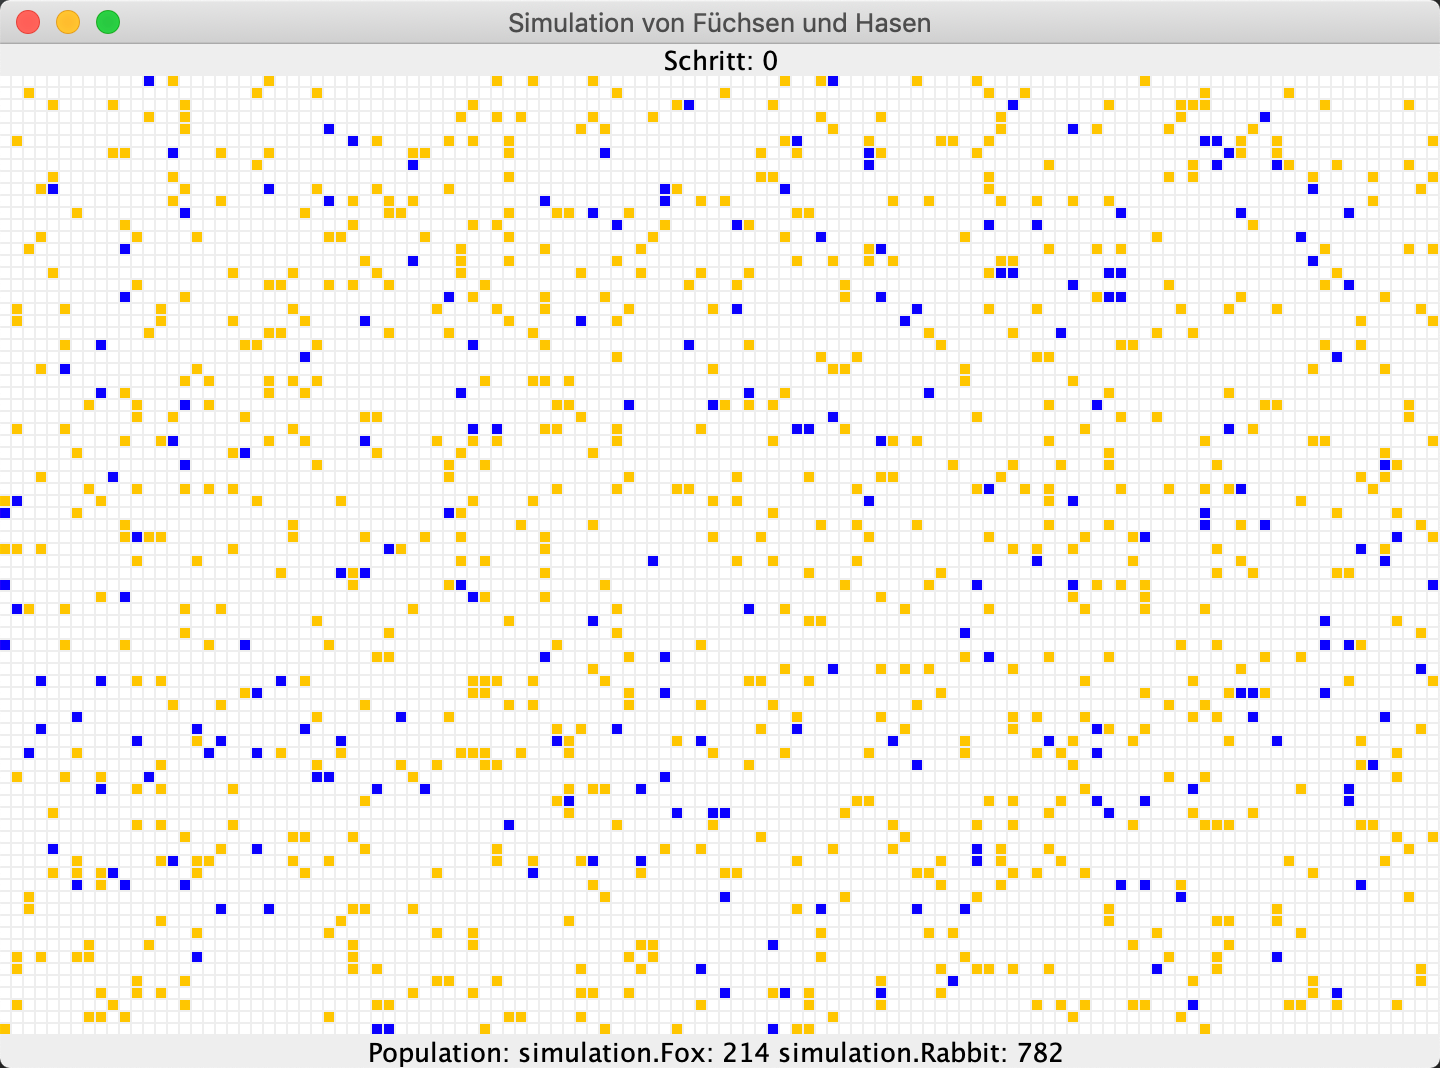
\includegraphics[height=7cm]{images/simulation-field.png}}
            \only<2>{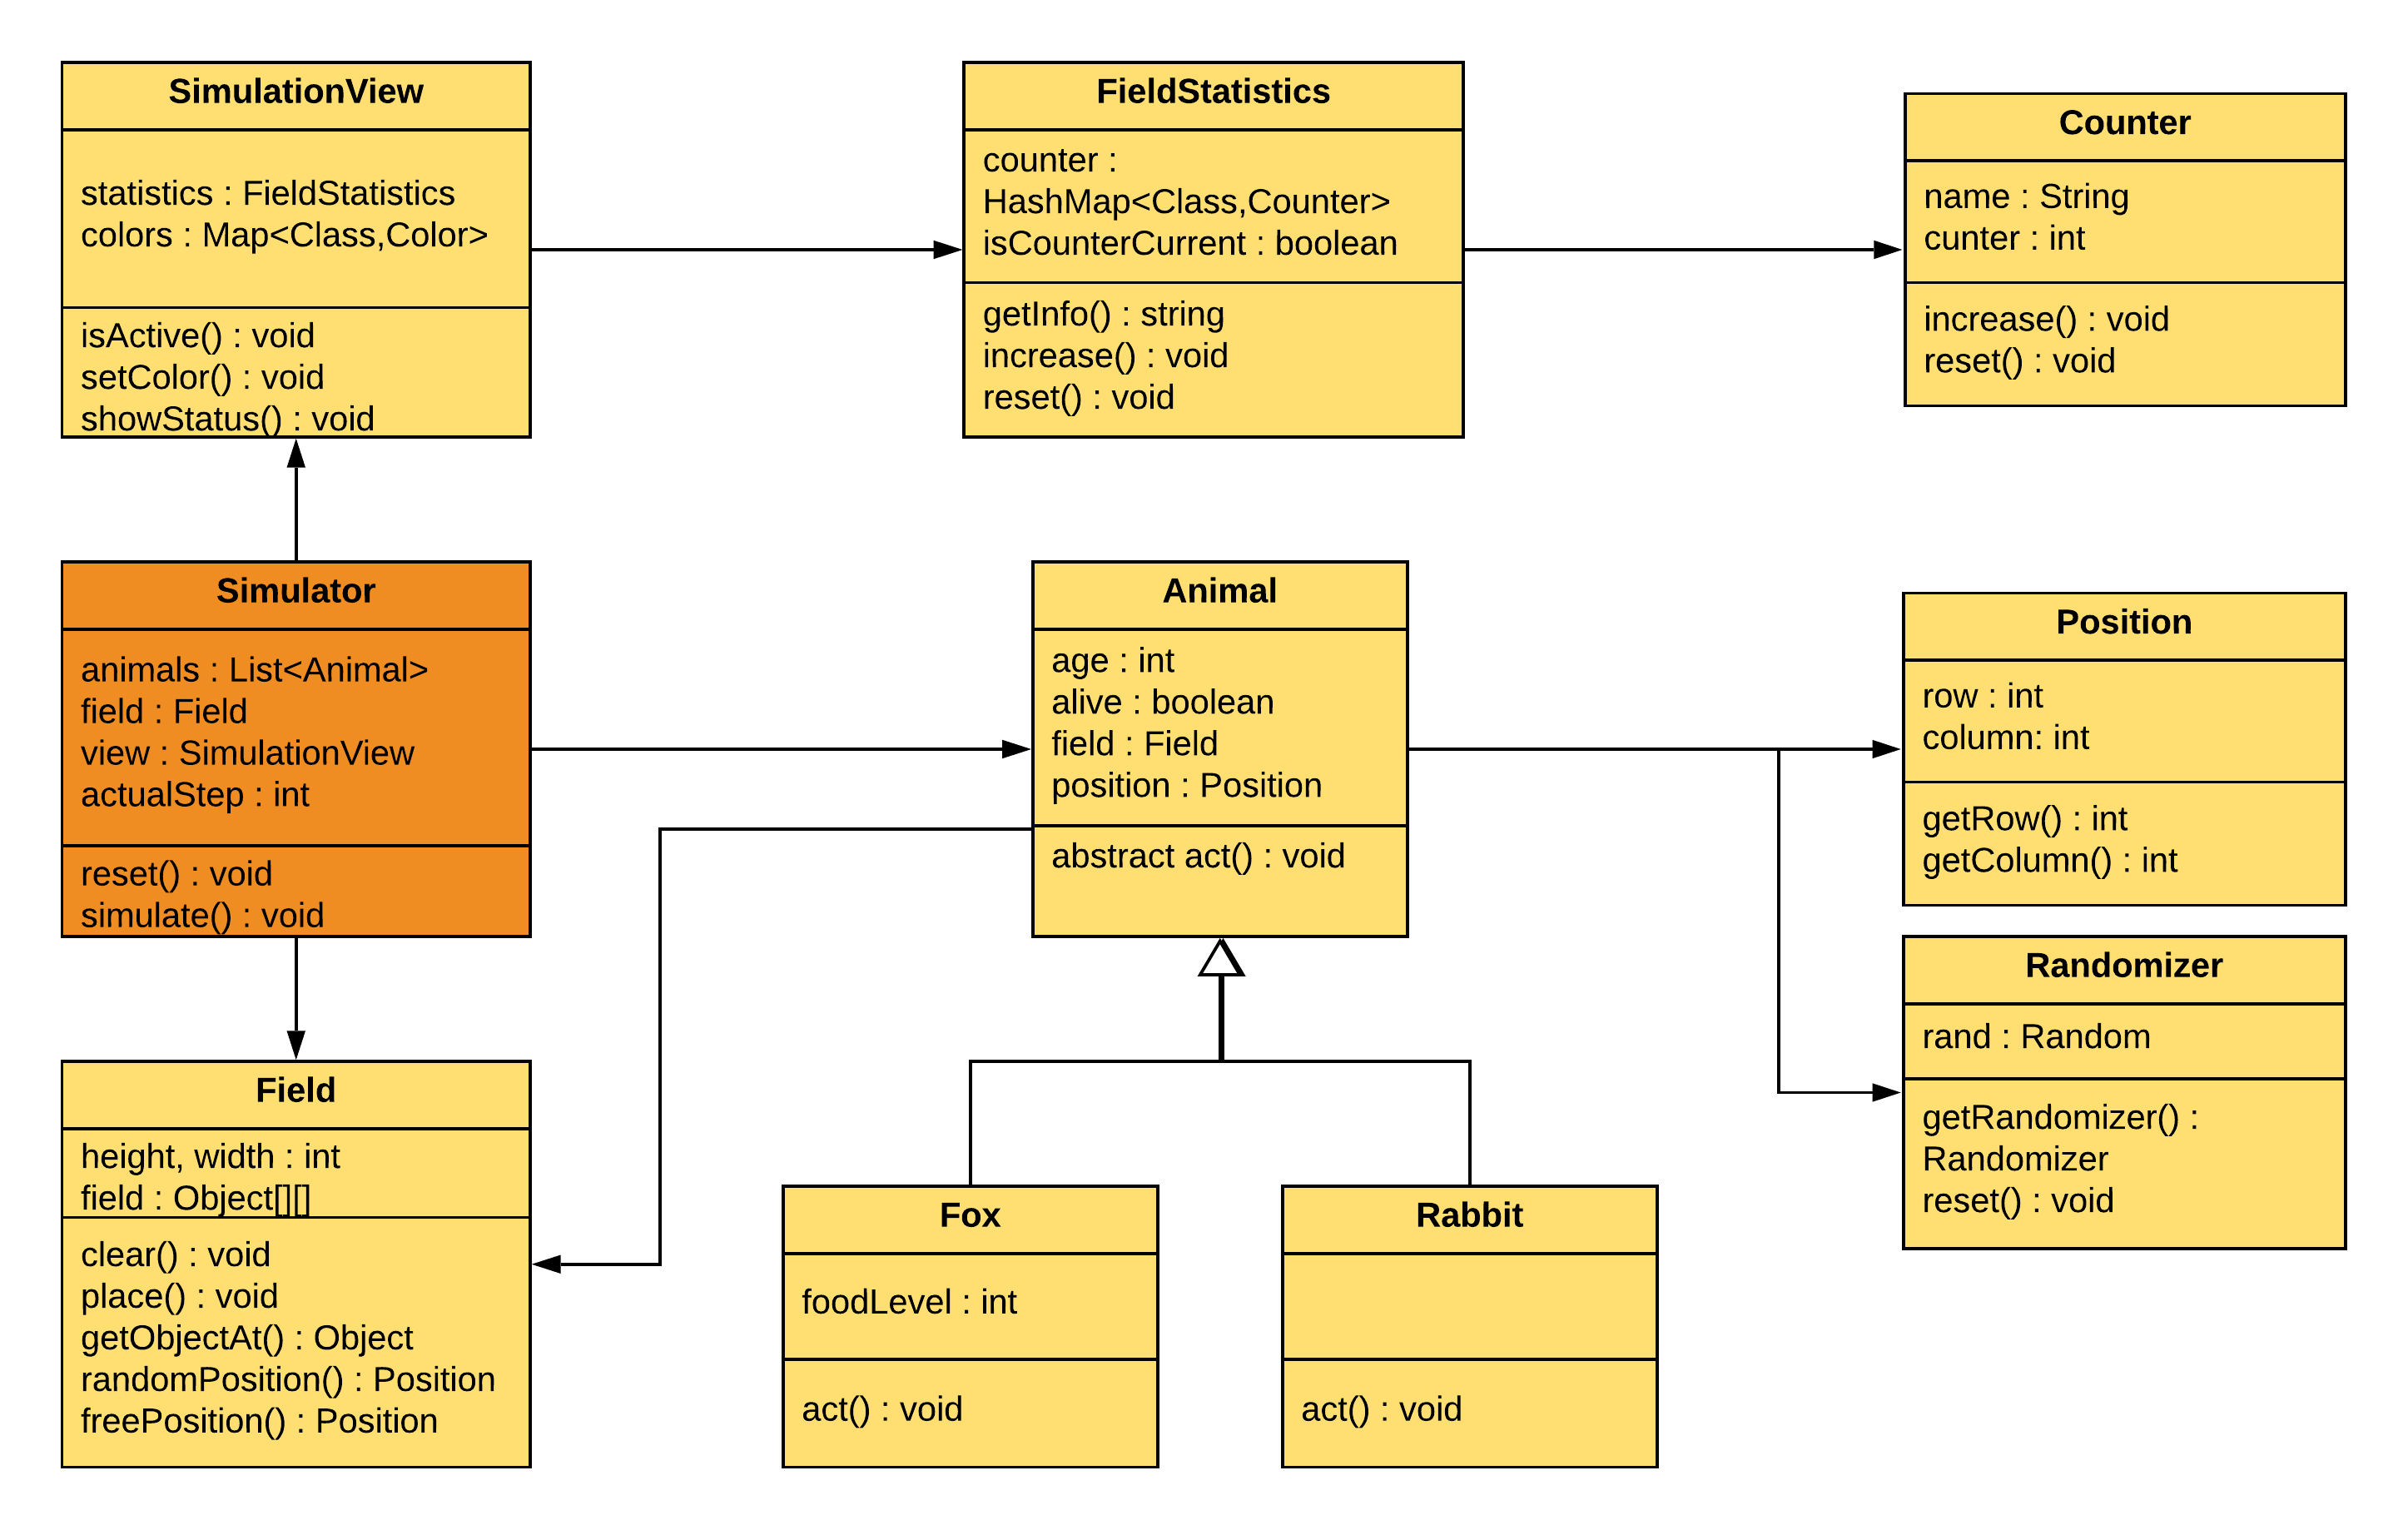
\includegraphics[height=7cm]{images/simulation-diagram.png}}
        \end{center}
    \end{figure}

\end{frame}
\mode*

\image{simulation-diagram}{Das Projekt Füchse und Hasen}

In dieser Simulation betrachten wir die Population von Füchsen und Hasen
in einem abgeschlossenen Feld. Sie ist ein Beispiel für sogenannte
\emph{Jäger-Beute-Simulationen}. Die zentralen Klassen für unser Beispiel
sind \textbf{Simulator}, \textbf{Animal} und die entsprechenden Spezialisierungen
\textbf{Fox} und \textbf{Rabbit}.

In Abbildung~\ref{fig:simulation-diagram} auf Seite~\pageref{fig:simulation-diagram}
ist das zugehörige Klassendiagramm abgebildet.

Die Klasse \textbf{Simulator} stellt den Anfangszustand der Simulation her
und kontrolliert ihren Ablauf. Der Simulator hält Sammlungen von Füchsen und
Hasen gibt diesen Tieren wiederholt die Möglichkeit, einen Schrittt ihres
Lebenszyklus zu durchleben. In jedem Schritt darf jeder Fuchs und jeder
Hase die Aktionen durchführen, die charakteristisch sind für sein Verhalten.
Nach jedem Scrhritt wird der aktuelle Zustand des Feldes auf dem Bildschirm
angezeigt.

Zusammenfassung der Funktionen der vorhandenen Klassen:

% -------------------------------------
\begin{frame}[fragile]
    \frametitle<presentation>{Beschreibung der Klassen}

    \begin{itemize}
        \item\textbf{Field} repräsentiert ein zweidimensionales begrenztes Feld.
            \mode<article>{Das Feld besteht aus einer festgelegten Anzahl von
                Positionen, die in Zeilen und Spalten angelegt sind. Eine
                Position kann von höchstens einem Tier eingenommen werden.
                Jede Position im Feld hält eine Referenz auf ein Tier oder
                ist leer.}
        \item\textbf{Position} repräsentiert eine zweidimensionale Position
            innerhalb des Feldes.
            \mode<article>{Eine Position wird durch einen Zeilen- und
                Spaltenwert definiert.}
        \item Die Zufallssteuerung (\textbf{Randomize}) gibt uns eine gewisse
            Kontrolle über diejenigen Aspekte der Simulation, die auf
            Zufallszahlen basieren (z.B.~die Geburt neuer Tiere).
        \item Die Klassen \textbf{SimulationView}, \textbf{FieldStatistics} und
            \textbf{Counter} kümmern sich um die grafische Darstellung
            der Simulation.
            \mode<article>{Die Ansicht der Simulation zeigt den Zustand des
            Feldes und der Zähler für die beteiligten Arten (die Anzahl der
            Füchse und Hasen).}
    \end{itemize}
\end{frame}

\begin{Exercise}[%
title={Verstehen der Simulation},
label={ex:simulation}]

    \begin{ExePart}
        Erzeugen Sie ein \textbf{Simulatior} Objekt mit dem parameterlosen
        Konstruktor, so dass der Anfangszustand der Simulation
        (Schritt: 0) angezeigt wird. Die zahlreichen Rechtecke repräsentieren
        die verschiedenen Tierarten (Füchse und Hasen).

        Ändert sich die Anzahl der Füchse, wenn Sie die Methode
        \textbf{simulateStep()} einmal aufrufen?
    \end{ExePart}


    \begin{ExePart}
        Ändert sich die Anzahl der Füchse mit jedem Schritt? Welche natürlichen
        Prozesse werden Ihrer Meinung nach modelliert, die die Anzahl der Füchse
        erhöhen oder reduzieren?
    \end{ExePart}


    \begin{ExePart}
        Rufen Sie die Methode \textbf{simulate()} so auf, dass ein grösserer
        Zeitraum von 50 bis 100 Schritten simuliert wird.

        Verändern sich die Zahlen der Füchse und Hasen in ähnlicher Weise?
    \end{ExePart}


    \begin{ExePart}
        Welche Änderungen beobachten Sie, wenn Sie die Simulation für einen sehr
        grossen Zeitraumlaufen lassen, etwa für 4'000 Schritte?
    \end{ExePart}

\end{Exercise}
